\documentclass[conference]{IEEEtran}
\usepackage[T1]{fontenc}
\IEEEoverridecommandlockouts
% The preceding line is only needed to identify funding in the first footnote. If that is unneeded, please comment it out.
\usepackage{cite}
\usepackage{amsmath,amssymb,amsfonts}

\usepackage[linesnumbered,ruled,vlined]{algorithm2e}
\DontPrintSemicolon
\usepackage[hidelinks]{hyperref}
\usepackage[noabbrev,capitalize]{cleveref}
\usepackage{array, booktabs, makecell}
\usepackage{graphicx}
\usepackage{textcomp}
\usepackage{xcolor}
\usepackage{caption}
\usepackage{subcaption}

\usepackage{tikz}
\usetikzlibrary{trees}

\newcommand\norm[1]{\left\lVert#1\right\rVert}
\def\BibTeX{{\rm B\kern-.05em{\sc i\kern-.025em b}\kern-.08em
    T\kern-.1667em\lower.7ex\hbox{E}\kern-.125emX}}

\graphicspath{../}
\hypersetup{
    colorlinks=true,
    linkcolor=black,
    filecolor=black,      
    citecolor=black,
    urlcolor=blue,
    pdfpagemode=FullScreen,
    }

\begin{document}

\title{Parallel Huffman Coding}

\author{\IEEEauthorblockN{Francesco Bozzo}
    \IEEEauthorblockA{\textit{DISI, University of Trento} \\
        Trento, Italy\\
        francesco.bozzo@studenti.unitn.it\\
        229312}
    \and
    \IEEEauthorblockN{Michele Yin}
    \IEEEauthorblockA{\textit{DISI, University of Trento} \\
        Trento, Italy\\
        michele.yin@studenti.unitn.it\\
        229359}
}

\maketitle

% add page number
\thispagestyle{plain}
\pagestyle{plain}

\begin{abstract}
    This report aims to explain the design of a parallel encoding and decoding Huffman algorithm. The application is developed with the C99 programming language, using MPI for multiprocessing and OpenMP for multithreading to scale horizontally with increasing hardware resources. Our tool is both able to exploit multiprocessing to process concurrently multiple files, and to split the Huffman coding of the same file among multiple threads.

    Comparing this tool with other online implementations, we can state that\dots
\end{abstract}

\begin{IEEEkeywords}
    Huffman, MPI, OpenMP, High Performance Computing
\end{IEEEkeywords}

\section{Introduction}
The \emph{Huffman algorithm} is designed to find a more convenient bit representation, to store data through lossless compression. Instead of considering groups of eight bits to encode data, the Huffman algorithm uses variable length sequences of bits defined as \emph{alphabet}.

The objective of our work is to build a scalable Huffman encoder and decoder that are able to scale according to the provided hardware resources. Moreover, the application should handle both single files and nested folders properly.

Even if nowadays the Huffman algorithm is mainly used for teaching purposes, its prefix mechanism is still part of many notable standards, such as Deflate (PKZIP's algorithm), JPEG, and MP3 compression algorithms. For this reason, there are no state-of-the-art online-available implementations to compare our tool with. In fact, differently from our work, many of the tools we found are not built considering low-level optimizations (such as to use in-memory buffers to improve I/O timings) or non-essential features (such as folders and big files handling).

\section{The Huffman algorithm}
The Huffman algorithm has the objective of finding a more convenient bit representation to store information through lossless compression. Instead of considering groups of eight bits as the way to encode data, the Huffman algorithm uses variable-length sequences of bits with prefixes defined as \emph{alphabet}.

\subsection{Priority Queue}
The Huffman algorithm uses a minimum priority queue to build its alphabet efficiently. This specific data structure ensures logarithmic insertion and deletion time with respect to its size.
We implemented the minimum priority queue by using a minimum heap. Practically speaking, to implement the min-heap tree, we used a standard C array ensuring that the min-heap property still holds at every insertion and deletion:
\begin{equation}
    A[i] \le A[l(i)], A[i] \le A[r(i)]
\end{equation}
where \(A[i]\), \(A[l(i)]\), \(and A[r(i)]\) are respectively a node, its left child, and its right child in a min-heap tree.

To implement the priority queue also a parallel approach has been considered \cite{BRODAL19984}, but since it contains only 256 elements (1 byte), we did not consider it too important in terms of performance.

\subsection{Encoding}
The Huffman encoding procedure makes use of a minimum priority queue to build its alphabet efficiently. The idea is to build a tree similar to \cref{fig:tree} that defines all the variable-length prefix sequences of bits: these sequences are represented by the path from the tree root to a leaf. Using a greedy approach, the Huffman encoding ensures that the less frequent a byte is in a file, the more probable is to have a longer Huffman representation, which means that his path from the root to its specific leaf is longer.

Once having computed the frequencies for each one of the 256 different bytes in a file, the Huffman algorithm populates a min priority queue with Huffman tree nodes storing the byte value and its frequency. Successively, it removes the least two frequent bytes from the queue, creates a new node with children the two extracted nodes, assigns to it a dummy character and the sum of the frequencies of its two children, and inserts it into the min priority queue. After \(n-1\) iterations, the last node is the root of the Huffman tree \cite{bertossi2010algoritmi}. \Cref{alg:buildtree} explains in the detail this procedure.
\begin{algorithm}
    \caption{Build the Huffman tree}\label{alg:buildtree}

    \SetKwData{Q}{Q}\SetKwData{z1}{z1}\SetKwData{z2}{z2}\SetKwData{z}{z}
    \SetKwFunction{insert}{insert}\SetKwFunction{deleteMin}{deleteMin}
    \SetKwInOut{Input}{input}\SetKwInOut{Output}{output}
    \SetKwFor{}{}{}{}

    // Populate the min priority queue with characters and their frequencies\;
    \For{\(i=1\) \KwTo \(n-1\)}{
        Q.insert(f[i], Tree(f[i], c[i]))\;
    }
    // Repeat until the queue has only a single element left\;
    \For{\(i=1\) \KwTo \(n-1\)}{
        // Get the two least frequent nodes\;
        z1 = Q.deleteMin()\;
        z2 = Q.deleteMin()\;

        // Create an inner tree node and insert it into the queue\;
        z = Tree(z1.f + z2.f, null)\;
        z.left = z1\;
        z.right = z2\;
        Q.insert(z.f, z)\;
    }

    // The last element in the queue is the root of the Huffman tree\;
    \Return{Q.deleteMin()}\;
\end{algorithm}

Once built the Huffman tree, it is possible to generate the Huffman alphabet visiting the tree using a DFS algorithm, assigning 0 to each left-child traverse and 1 for the right one as presented in \cref{alg:encode}. Finally, it is possible to compress the file by creating a stream of bits corresponding to its content using the Huffman alphabet.

\begin{algorithm}
    \caption{Encode using Huffman tree}\label{alg:encode}
    \While{not eof()}{
        bit = read()\;
        \eIf{bit == 0}{
            encode(node.left)\;
        }{
            encode(node.right)\;
        }
        \If{node is leaf}{
            \Return{node.value}\;
        }
    }
\end{algorithm}

\begin{center}
    \begin{figure}
        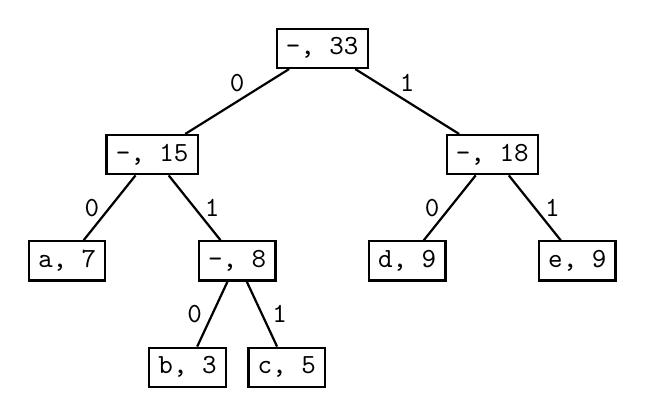
\begin{tikzpicture}
            [
                level distance=1.5cm,
                level 1/.style={sibling distance=4.8cm},
                level 2/.style={sibling distance=2.4cm},
                level 3/.style={sibling distance=1.4cm},
                thick,
                font=\ttfamily\bfseries, scale=0.9
            ]
            \tikzset{
                treenode/.style = {rectangle, draw=black, align=center,minimum width=0.75cm},
                edgestyleL/.style = {midway,left,draw=none},
                edgestyleR/.style = {midway,right,draw=none}
            }
            \node [treenode] (T) {-, 33}
            child { node[treenode] (L) {-, 15}
                    child { node[treenode] (LL) {a, 7} edge from parent node[edgestyleL] {0} }
                    child { node[treenode] (LR) {-, 8}
                            child { node[treenode] (LRL) {b, 3} edge from parent node[edgestyleL] {0} }
                            child { node[treenode] (LRR) {c, 5} edge from parent node[edgestyleR] {1} }
                            edge from parent node[edgestyleR] {1}
                        }
                    edge from parent node[edgestyleL,above] {0}
                }
            child { node[treenode] (R) {-, 18}
                    child { node[treenode] {d, 9} edge from parent node[edgestyleL] {0}}
                    child { node[treenode] {e, 9} edge from parent node[edgestyleR] {1}}
                    edge from parent node[edgestyleR,above] {1}
                }
            ;
        \end{tikzpicture}
        \caption{An example of Huffman tree.}
        \label{fig:tree}
    \end{figure}

\end{center}

\subsection{Decoding}
Once having the encoded file and the Huffman tree, it is straightforward to decompress the file to its original shape. The prefix alphabet ensures to have that it is possible to visit the tree using a DFS approach and get a unique decoded version of the file using an approach similar to \cref{alg:encode}.

\section{Serial Huffman implementation}
To be able to implement the Huffman encoding and decoding algorithm, several things have been taken into account.
\begin{itemize}
    \item The byte frequencies computed during the encoding process are saved in the compressed file. In this way, the decoding procedure can easily rebuild the Huffman tree.
    \item Both the encoding and decoding procedures make use of buffers to improve I/O performance: the streams of bytes are first written inside the buffer and then saved on the disk.
    \item The encoding procedure works with chunks of \(4096\) bytes. This ensures that the tool can handle even large files when dealing with bit buffers. The decoding procedure deals with chunks of maximum size of \(4096*32\) bytes, since the maximum length of a Huffman tree traverse from root to leaf is of 256 bits. As explained later, dealing with chunks makes handy the parallel implementation of the encoding and decoding algorithms.
    \item In the encoded file, the chunk offsets are saved at the end of the file: this ensures that the compressed stream of prefixed sequences of bits is still meaningful.
\end{itemize}

\section{Parallel Huffman Implementation}
To parallelize our algorithm over threads and processes, we decided to follow this structure
\begin{itemize}
    \item multiple processes to process groups of file and folders separately;
    \item multiple threads to process different chunk of the same file in parallel.
\end{itemize}

There are a few motivations to our choice. Mainly are:

\begin{itemize}
	\item In most operating systems a file is a resource that the OS gives to a single process. We wanted to follow a similar design philosphy.
	\item Most operating system can allow multiple processes to open the same file in reading mode, but few allow to multiple processes to open the same file in writing mode. This is because that leads to potentially concurrency and data integrity issues.
	\item Because threads of the same process share the address space, we can avoid the expensive data transfer across processes by parallelizing a single file using threads instead of processes. 
\end{itemize}

The parallel algorithm follows the same exact procedure as a serial version.

However we decided to process a file using multiple threads.

That means that a single file is divided in chunks of a fixed size. 

Then the program forks the number of threads we intented.

One of them reads a number of chunks equal to the number of threads. When it's done reading the chunks, all threads can work on the processing.

Every chunk is processed by a single thread. 

When all threads are done processing their chunks, a thread writes the completed chunks to file. Because all threads share a memory space there is no need to perform data transfer.


The procedure is the same in both encoding and decoding. Also counting occurences follow a similar architectures, but without the write operations.





For multiple files, the rank 0 crawls all the files in the input directory. Then it opens all the files and reads their size. Then it creates a priorityQ where each item is a process and it inserts files in the priorityQ and updates the priority with the file size. This way we can ensure a proper almost equal work division among different processes.

When all this is done, the rank 0 sends the list of files to each process and then each process starts to work indipendetly on it's own list of files.


Implementation and detailed notes

We found that a size of 4096 bytes had  the best IO times, probably due to the fact that 4096B is the size of a page in most Linux based operating systems. The last chunk may be smaller.

We tried to parallelize the IO, having multiple threads that read it's own chunk. We found that the standard File Descriptor provided by C language has a lock to guarantee thread safety. However that slows down the reads significantly. Instead we tried using multiple file descriptors to circumvent this limitation. However we found no improvement over a serial read done by one thread for all the threads in it's team. This is likely because the OS schedules the IO requests and serves them one at the time, resulting in impossible truly parallel IO.

We also tested a architecture where we had two dedicated threads to IO, one for reading and one for writing chunks. This way the idea was that whenever a chunk was processed, the IO thread would read and write the related chunks, without delays due to the IO, and synchronizing the IO with locks to prevent inconstenstencies. However we found that this approach was a waste  of resources, as the IO on the cluster is extremely fast (5GB+/s) and would result in the IO threads being idle most of the time.

The schema is presented in Figure here

\section{Performance and benchmarking}
In this section we are going to discuss the performance evaluation of our algorithm. We start from evaluating some other implementations of Huffman algorithm and then focus on the analysis of our own implementation. 

We include in this section some graphs and statistics, but all detailed results are included in the appendix at the end this report.
\subsection{Setup}
All the tests were performed on the HPC2 cluster of the University of Trento. To reduce as much as possible the I/O timings, which are crucial of our application, jobs were run in a very specific setting:

\begin{itemize}
	\item Threads are allocated in the same node and, if possible, on the same socket to guarantee fast communication between them. This has been achieved by using the MPI option \verb|--map-by|.
	\item Processes are allocated in different nodes, by using the PBS directive \verb|place=scatter:excl|. This because in our application different processes do not communicate very often between each other, but they just split their work and use the file-system. We also tested \verb|place=pack:excl| but found worse results.
\end{itemize}

The provided timings are obtained by averaging the result of three runs with the exact same configurations: this helps to minimize the effect random variance between runs due to potential hardware congestion.
Each job has been submitted to the cluster individually, waiting for the previous to finish preventing hiccups due to multiple instances of the program trying to access the same file-system resource, which we noticed to greatly affect I/O times.

We extensively verified the correctness of our algorithm by encoding and then decoding a file, then comparing the decoded result to the original file by using the \verb|diff| command. Moreover, Valgrind has been used to spot any memory leaks that could cause runtime errors.

\subsection{Datasets}
The evaluation dataset has been randomly generated by using a simple C program: we created text files with character frequencies that follow the occurrences of the letters in English language. Although for benchmarking we are only using ASCII characters, please note that our algorithm reads bytes of data and can therefore work with any file.
The dataset is composed by files of increasing size: 1 MiB, 5 MiB, 10 MiB, 50 MiB, 100 MiB, 500 MiB, 1 GiB, 5 GiB, and 10 GiB. This should be enough range to understand how different algorithms scale with increasing file sizes.

Secondly, because our algorithm also works with many files at once, we chose some GitHub repositories as benchmark: Numpy\cite{2020NumPy-Array}, PyTorch \cite{Paszke_PyTorch_An_Imperative_2019} and Linux kernel \cite{linux}. They are respectively $\sim$ 30 MiB,$\sim$ 200 MiB and $\sim$ 1.3 GiB of total size, with about $\sim$ 2.000, $\sim$ 12.000, and  $\sim$ 80.000 files, which on average are each 16MiB.

% Considering the dataset sizes and amount testing we have done, we estimate to have accessed the disk (both read and writes) for about $\sim$ 6 TiB of data for our whole benchmark analysis.


\subsection{Multithreading evaluation}
In this section we evaluate our algorithm on single files, by using multithreading and testing our parallelization performances with an increasing number of threads.

With small files (i.e. less than a few MiBs) the algorithm is actually slower with more threads. This is likely because the data is not large enough to offset the cost of forking multiple threads. Considering the cost parallel processing, we highly suggest not doing parallelization for small files. However, when the data is large enough our multithreaded approach scales up. With the largest file (10 GiB) our algorithm has an efficiency of 93\% when tested with 4 threads. This number steadily decreases with the number of threads, and we hit 16\% with 64 threads.

The same issue is even more visible by looking at one implementation we found on GitHub that uses only MPI for parallelization\cite{HuffmanCodingMPICUDA}: with many processes, while with large files (even though it does not work with files bigger than $\sim$500 MiB) it performs better than our implementation, with small files it is not able to scale. This is happening due to the overhead of splitting small files among too many processes. This fact can be observed also by looking at \cref{fig:ours-vs-online}.
\begin{figure}
	\centering
	\includegraphics[width=1\linewidth]{"../imgs/our vs online 7"}
	\caption{Ours vs online implementation}
	\label{fig:ours-vs-online}
\end{figure}
Additionally, please note that our tool is heavily limited by the cluster I/O: especially writes to disk require a considerable amount of time. As a proof of this, if we consider only the processing section of our algorithm, and ignore the time required by the \verb|fflush()| operation before \verb|fclose()|, we see significantly decreased times. Although we start from similar efficiency at low threading, we achieve a 41\% efficiency with 64 threads in this case. % if we consider only CPU time, which does not count the time spent waiting in I/O, we get very promising results.

\begin{figure}
	\centering
	\includegraphics[width=1\linewidth]{"../imgs/Flush vs non Flush"}
	\caption{Encoding times with and without the flush()}
	\label{fig:flush-vs-non-flush}
\end{figure}

We also noticed worse times in the decoding procedure with respect to encoding. This is probably due to the fact that the tool is reading fixed chunks of 4096 bytes in encoding, but during decoding the chunk can have a variable length.
Moreover, by executing another implementation found on GitHub \cite{HuffmanParallel2}, we found that reading and writing buffers to the disk (and not single bytes) can obtain improvement very similar to one order of magnitude.

As already discussed previously, we also tested a version on a lock-based synchronization instead of barriers. Although theoretically we should get better results, in practice we obtain almost equal performances across the board, with only the largest files having some significant difference. This difference is greater in decoding than in encoding.
% \begin{figure}
% 	\centering
% 	\includegraphics[width=1\linewidth]{"../imgs/Barrier vs Locks encoding"}
% 	\caption{Barrier vs Lock based synchronization performance}
% 	\label{fig:barrier-vs-locks-encoding}
% \end{figure}

\begin{figure}
	\centering
	\includegraphics[width=1\linewidth]{"../imgs/encoding speedup wide"}
	\caption{Encoding speedup}
	\label{fig:encoding-speedup}
\end{figure}
\begin{figure}
	\centering
	\includegraphics[width=1\linewidth]{"../imgs/encode efficiency wide"}
	\caption{Encoding efficiency}
	\label{fig:encoding-efficiency}
\end{figure}


\subsection{Multiprocessing}
We tested on different folders the parallelization performances of our algorithm. Theoretically, it should scale very well with increasing number of processes and files, because once the main process sends the list of files to encode to each process there is no further communication between different processes. However, we find that real world results are different.

While we do not expect much performance improvement by the number of threads, because the files are on average very small, we should get better results by using many processes. In reality, our testing shows that this is not the case, probably due to the slow cluster I/O. When tested on a local machine (MacBook A2442) with one thread and 1,2,4 processes, we find that our algorithm does indeed scale with the number of processes.
We also find that \verb|scatter| scales better than \verb|pack|, probably because with \verb|scatter| we are not limited by the I/O of a single node.
\begin{figure}
	\centering
	\includegraphics[width=1\linewidth]{"../imgs/linux speedup"}
	\caption{Linux speedup for different placing strategies}
	\label{fig:linux-scatter-pack}
\end{figure}

% \subsection{Memory, storage and other considerations}
% We also find that we achieve on average 48\% compression rate of our synthetic data. Instead, on Linux kernel, because contains more varied data which consists of mostly code, we achieve a lower 62\% compression rate. Testing on other already compressed data as \verb|.zip| or \verb|AV1| resulted in a compression rate of 100\%.

\section{Conclusions}
To conclude.


\bibliography{bibliography.bib}{}
\bibliographystyle{IEEEtran}

\end{document}
